%\documentclass[handout]{beamer}
\documentclass[presentation]{beamer}

\usecolortheme{UTUaaro}
 
\usepackage[utf8]{inputenc}
\usepackage[UKenglish]{babel}
\usepackage{booktabs}
\usepackage{caption}
\usepackage{subcaption}
\usepackage{graphicx}
\usepackage{amsmath}
\usepackage{amsfonts}
\usepackage{amssymb}
\usepackage{fancybox}
\usepackage{epstopdf}

\usepackage{pdfpc-commands}

\usepackage{lipsum} % for template demonstration

% complying UK date format, i.e. 1 January 2001
\usepackage{datetime}
\let\dateUKenglish\relax
\newdateformat{dateUKenglish}{\THEDAY~\monthname[\THEMONTH] \THEYEAR}


\institute{
\includegraphics[height=1.5cm]{UTU_logo_RGB_EN.pdf}}


% -----------------------------------------------------------------------------
% vähän tekstiä per slide, paljon yleistajuisia pointteja

% pointeja:
% tilastollinen koneoppisen teemoja:
% paljon samanlaisia yksinkertaisia palasia pystyvät mallintamaan monimutkaisia asioita
% tilatotieteellinen päättely automatisoituna?
%
% ei ihmis- tai eläinkognition/älyn mallintamista, ainakaan kovin usein
% -> neuroverkotkin lähinnä inspiroituneita kuin edes abstrakteja malleja aivokuoresta
%

% tapausesimerkki: % https://www.helsinki.fi/fi/uutiset/terveys/suomalaistutkijat-kehittivat-tekoalyalgoritmin-aivovammapotilaiden-tehohoitoon

% aiheet
% 1. logistinen regressio? muurahainen.
% 2. neuroverkko. limasieni? termiittikeko.

% Aikatauluts + kalvot
% johdanto: 5 min
%   Tekoälystä puhutaan paljon. Ehkä joskus jossain on jotain, mutta minun puhun
%       algoritmeista 
%
%   mitä tilastollinen oppiminen tarkoittaa:
%       
%   kuinka algoritmin onnistumista mitataan
% lineaarinen regressio: 10 min
% logistinen regressio: 10 min
% konvolutiivinen neuroverkko: 10 min
% (päätöspuu -> satunnaismetsät: 10 min)
% yhteenveto: 5 min
% https://link.springer.com/article/10.3758%2Fs13420-020-00410-z
% = 40 min

% laskuesimerkkien toteutus
% optio 1: toteuta Julialla (opin Juliaa!)
% optio 2 jos feilaa: Python ja scikit (kertaan Python-Scikit!)

% https://github.com/bensadeghi/DecisionTree.jl
% https://github.com/JuliaStats/GLM.jl
% https://github.com/FluxML/model-zoo/
% jas nns, also alternative logres. https://github.com/FluxML/model-zoo/blob/master/other/iris/iris.jl

\title{Kurkistus tilastollisesti oppivien koneiden eläintarhaan}

% tavoitemitta: 30-45 min + keskustelu
\subtitle{Studia Varjomafia 4, Terrakoti}

\author{Aaro Salosensaari aaro.salosensaari@utu.fi}

\date{22.2.2020}

\begin{document}
 
\frame{\titlepage}

\begin{frame}{Mikä on tilastollisesti oppiva kone?}
    
\end{frame}

\begin{frame}{Algoritmi}
	\begin{columns}[]
		\column{0.0125\textwidth}
		\column{0.4875\textwidth}
			\centering
			\begin{figure}
				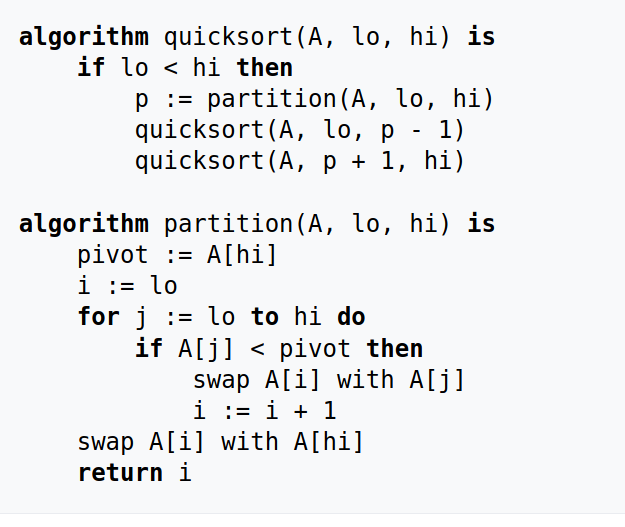
\includegraphics[width=\textwidth]{quicksort.png} \
				% remove the 'draft' keyword, when replacing with final figure!
				% \inlineMovie[loop&autostart&start=5&stop=12]{apollo17.avi}{apollo17.jpg}{height=0.7\textheight}
				\caption{Caption of Figure C}
			\end{figure}
		\column{0.4875\textwidth}
		    \centering
		    \inlineMovie[loop&autostart]{Sorting_quicksort_anim.gif}{sorting_gif-0.png}{width=\textwidth}
		\column{0.0125\textwidth}
	\end{columns}
    \includegraphics[]{}
\end{frame}


%\begin{frame}{Contents}
%
%\begin{itemize}
%    \item point A
%    \item point B
%\end{itemize}
%
%\end{frame}

%\begin{frame}{Frame with lots of text}
%    \lipsum[1-1]
%\end{frame}

%\begin{frame}
%	\frametitle{Text and Figure aside}
%	\begin{columns}[]
%		\column{0.0125\textwidth}
%		\column{0.4875\textwidth}
%			\centering
%			\begin{figure}
%				%\includegraphics[draft,width=\textwidth]{fooC.pdf} \
%				% remove the 'draft' keyword, when replacing with final figure!
%				\caption{Caption of Figure C}
%			\end{figure}
%		\column{0.4875\textwidth}
%			Some text and a bullet point list
%			\begin{itemize}
%				\item ItemA
%				\item ItemB
%				\item ItemC
%				\item ItemD
%			\end{itemize}			
%		\column{0.0125\textwidth}
%	\end{columns}
%\end{frame}


\begin{frame}{References}
    ...
\end{frame}

\end{document}

